\documentclass{scrreprt}

\usepackage{aligned-overset}
\usepackage{amsmath}
\usepackage{amssymb}
\usepackage{bm}
\usepackage[shortlabels]{enumitem}
\usepackage{hyperref}
\usepackage[utf8]{inputenc}
\usepackage{mathtools}
\usepackage{physics}
\usepackage{tabularx}
\usepackage{titling}
\usepackage{fancyhdr}
\usepackage{xfrac}
\usepackage{pgfplots}

\definecolor{light-gray}{gray}{.9}

\pgfplotsset{compat = newest}
\usetikzlibrary{intersections}
\usetikzlibrary{patterns}
\usepgfplotslibrary{fillbetween}

\author{Karsten Lehmann}
\date{SoSe 2021}
\title{Übung 07 Analysis - Weiterführende Konzepte}

\pagestyle{fancy}
\fancyhf{}
\lhead{\thetitle}
\rhead{\theauthor}
\lfoot{\thedate}
\rfoot{Seite \thepage}

\begin{document}
\fcolorbox{black}{light-gray}{\begin{minipage}{\textwidth}
    \textbf{Linearer Operator} (auch lineare Abbildung) ist eine
    strukturerhaltende Abbildung zwischen Vektorräumen über einen
    gemeinsamen Körper.

    Seien $X, Y$ Vektorräume und $T \colon X \to Y$ eine Abbildung, dann heißt
    $T$ linearer Operator, wenn
    \begin{enumerate}
    \item $\forall x, y \in X$ und $\lambda \in \mathbb{R} \colon T(\lambda x) = \lambda T(x)$
    \item $\forall x, y \in X \colon T(x + y) = T(x) + T(y)$
    \end{enumerate}
\end{minipage}}

Sei $X, Y$ normiert, ein Operator $T \colon X \to Y$ linear.
\begin{enumerate}[(i)]
\item $T$ ist stetig $\iff$
\item $T$ ist in $0$ stetig $\iff$
\item $T$ ist beschränkt, d.h. $\exists c > 0 \forall x \in X\colon \norm{T_x}_y \leq c \norm{x}$
\end{enumerate}
\label{c_inf}
\[
  T \in \mathcal{L}\qty{X, Y} = \qty{T \colon X \to Y {\Big |} T \text{ ist linear stetig}} (*)
\]
\begin{flalign*}
  \norm{T} &= \inf\qty{c > 0 \, {\Big |} \text{ Es gilt } (*)} & \\
  &= \sup\qty{\frac{\norm{Tx}_y}{\norm{x}_x} \, {\Big |} \, x \ne 0} & \frac{\norm{T_x}_y}{\norm{x}_x} = \norm{T\qty(\frac{x}{\norm{x}_x})} \\
  &= \sup\qty{\norm{T_x}_y {\Big |} \norm{x}_x = 1} =  \sup\qty{\norm{T_x}_y {\Big |} \norm{x}_x \leq 1}
\end{flalign*}

$T \in \mathcal{L}\qty(\mathbb{R}^N, \mathbb{R}^M)$ und Basen $\phi$ auf
$\mathbb{R}^N$ und $\psi$ auf $\mathbb{R}^M$ seien gegeben.

$\Rightarrow$ Es gibt genau eine Matrix $A$, die die Koordinatenvektoren transformiert.

$x = \sum_{k=1}^N x_k \phi_k, \underline{x} = \qty{x_1, \ldots, x_n} T_x = \sum_{k=1}^N x_k T(\phi_k) = \sum_{j=1}^M y_i \psi_j, \underline{y} = \qty{y_1, \ldots, y_m}$

$\Rightarrow \underline{y} = A \cdot \underline{x}$

\paragraph{Aufgabe 1} Der Raum $\mathcal{L}\qty(\mathbb{R}^N, \mathbb{R}^M)$ kann mit
$R^{M \times N}$ identifiziert werden.
Sind Normen $\norm{\cdot}_{\mathbb{R}^N}$ und
$\norm{\cdot}_{\mathbb{R}^M}$ auf den Räumen $\mathbb{R}^N$ bzw.
$\mathbb{R}^M$ gegeben, so ist durch
\[
  \norm{A} \coloneqq \sup\qty{ \norm{A \cdot x}_{\mathbb{R}^M} {\Big |} \norm{x}_{\mathbb{R}^N} \leq 1}
\]
eine Operatornorm auf $R^{M \times N}$ definiert.
Die Räume $\mathbb{R}^N$ und $\mathbb{R}^M$ seien mit der $\norm{\cdot}_1$-Norm
versehen.
Beweisen Sie, dass sich als Operatornorm von $A \in R^{M \times N}$ die
sogenannte \textit{Spaltensummennorm} ergibt:
\[
  \norm{A} = \underset{k=1,\ldots,N}\sum_{j=1}^M \abs{a_{jk}} \text{ für alle } A \in \mathcal{L}\qty(\mathbb{R}^N, \mathbb{R}^M)
\]

\newpage
\textit{Lsg.} \\
Sei $T \in \mathcal{L}\qty(\mathbb{R}^N, \mathbb{R}^M)$ und $A$ die
Abbildungsmatrix bezüglich der Standardbasen.
\[
  \norm{x}_1 = \sum_{k = 1}^N \abs{x_k}, \quad \norm{y}_1 = \sum_{j = 1}^M \abs{y_j}
\]
Wir betrachten zunächst
\[
  A \cdot e^k =
  \qty(
    \begin{array}{ccccc}
      a_{11} & \ldots & a_{1k} & \ldots & a_{1N} \\ \\ \\
      \vdots & \vdots & \vdots & \vdots & \vdots \\ \\ \\
      a_{M1} & \ldots & a_{Mk} & \ldots & a_{MN}
    \end{array}
  )
  \cdot
  \qty(
    \begin{array}{c}
      0 \\
      \vdots \\
      0 \\
      1 \\
      0 \\
      \vdots \\
      0
    \end{array}
  )
  = \qty(a_{1k}, \ldots, a_{Mk}) \text{ (die $k$-te Spalte)}
\]
\[
  \Rightarrow \norm{A \cdot e_k}_1 = \norm{\qty(a_{1k}, \ldots, a_{Mk})}_1
  = \sum_{j = 1}^M \abs{a_{jk}}
\]
Wegen $\norm{e_k}_1 = 1$ folgt
$\frac{\norm{A \cdot e_k}_1}{\norm{e_k}_1} = \sum_{j = 1}^M \abs{a_{jk}}
\leq \sup\qty{\frac{\norm{A \cdot x}_1}{\norm{x}_1} {\Big |} x \in \mathbb{R^N}} = \norm{A}$
\begin{flalign*}
  \Rightarrow & \max_{k=1, \ldots, N} \sum_{j = 1}^M \abs{a_{jk}} \leq \norm{A} &
\end{flalign*}
Weiter gilt: Jedes $x \in \mathbb{R}^N$ besitzt eine eindeutige Darstellung der Form
$x = \sum_{k = 1}^N x_k e_k$
\begin{align*}
  \Rightarrow \norm{A \cdot x}_1 &= \norm{\sum_{k = 1}^N x_k \cdot A \cdot e_k}_1
  \leq \sum_{k = 1}^N \abs{x_k} \cdot \norm{A \cdot e_k}_1 \\
  &\leq \max_{k=1, \ldots, N}\norm{A \cdot e_k} \cdot \underset{= \norm{x}_1}{\underbrace{\sum_{k = 1}^N \abs{x_k}}} \\
  &= \max_{k=1, \ldots, N}\norm{A \cdot e_k} \cdot \norm{x}_1
\end{align*}
\begin{align*}
  \overset{x \ne 0}&\Rightarrow \frac{\norm{A \cdot x}_1}{\norm{x}_1} \leq \max_{k=1, \ldots, N}\sum_{j = 1}^M \abs{a_jk} \\
  \norm{A} &= \sup\qty{\frac{\norm{A \cdot x}_1}{\norm{x}_1} {\Big |}, \, x \ne 0 } \leq \max_{k=1, \ldots, N}\sum_{j = 1}^M \abs{a_jk} \\
\end{align*}
$\norm{A} = \max_{k = 1 \ldots N} \sum_{j = 1}^M \abs{a_{jk}}$ (die Spaltensummennorm)

\paragraph{Hausaufgabe 2} Seien $X, Y, Z$ normierte Räume und
$T \in \mathcal{L}\qty(X, Y)$ sowie $S \in \mathcal{L}\qty(Y, Z)$.
Dann gehört $S \circ T$ zu $\mathcal{L}\qty(X, Z)$.
Zeigen Sie folgende Ungleichung
\[
  \norm{S \circ T} \leq \norm{S} \cdot \norm{T}
\]

\textit{Lsg.} Eine Verkettung linearer Abbildungen ist ebenfalls linear.
Für $x \in X$ gilt
\begin{align*}
  \norm{(S \circ T) x} \in Z &= \norm{S(T x)} \in Z
                               \leq \norm{S} \cdot \norm{T x} \\
                             &\text{(\hyperref[c_inf]{Siehe $(*)$})} \\
                             &\leq \norm{S} \cdot \norm{T} \cdot \norm{x}_X
\end{align*}
\begin{align*}
  \overset{x \ne 0}\Rightarrow \frac{\norm{\qty(S \circ T)x}_Z}{\norm{x}_X}
  &\leq \norm{S} \cdot \norm{T} \\
  \norm{S \circ T} &= \sup\qty{\frac{\norm{\qty(S \circ T)x}_Z}{\norm{x}_X} {\Big |} \, x \ne 0} \\
  &\leq \norm{S} \cdot \norm{T}
\end{align*}

\paragraph{Hausaufgabe 3} $X = C([0, 1])$ sei mit der Supremumsnorm versehen.
Wir betrachten die Abbildungen $S, T \colon C([0, 1]) \to \mathbb{R}$,
definiert durch
\[
  T(f) \coloneqq \int_{0}^1 f(x)\,dx \text{ und }
  \overset{\delta-\text{Distribution}}{\overbrace{S(f) = f(0)}}
  \text{ für } f \in X
\]
Beweisen Sie, dass diese Abbildungen zu $\mathcal{L}\qty(X, \mathbb{R})$
gehören und berechnen Sie deren Normen, wenn auf $\mathbb{R}$ die Betragsmetrik
gegeben ist.

\textit{Lsg.} $S, T$ sind linear: Seien
$f, g \in C([0, 1]), \alpha, \beta \in \mathbb{R}$ gegeben.
Dann gilt:
\begin{align*}
  T(\alpha \cdot f + \beta \cdot g)
  &= \int_0^1 \qty\Big(\alpha \cdot f + \beta \cdot g)\qty\Big(x)\,dx \\
  &=\int_0^1 \alpha \cdot f(x) + \beta \cdot g(x)\,dx \\
  &= \alpha \int_0^1 f(x)\,dx + \beta \int_0^1 g(x)\,x  \\
  &= \alpha \cdot T(f) + \beta \cdot T(g) \\
  S(\alpha \cdot f + \beta \cdot g)
  &= \qty\Big(\alpha \cdot f + \beta \cdot g)\qty\Big(0)
    = \alpha \cdot f(0) + \beta \cdot g(0) \\
    &= \alpha \cdot S(f) + \beta \cdot S(g) \\
  \Rightarrow S, T & \text{ sind linear}
\end{align*}
\newpage
$S, T$ sind stetig mit $\norm{S} = \norm{T} = 1$: Für $f \in C([0, 1])$ gilt:
\begin{align*}
  \abs{T(f)} &= \abs{\int_0^1 f(x)\,dx} \leq \int_0^1
               \underset{\leq \norm{f}_{\infty}}{\underbrace{\abs{f(x)}}}\,dx
               \leq \norm{f}_{\infty} \int_0^1 dx = \norm{f}_{\infty} \\
  \overset{f \ne 0}&\Rightarrow \frac{\abs{T(f)}}{\norm{f}_{\infty}} \leq 1
                     \Rightarrow \norm{T} \leq 1
\end{align*}
\begin{flalign*}
  \text{Für $f_0(x) = 1, x \in \qty[0, 1]$, gilt $\abs{T(f)} = \int_0^1 1\,dx = 1$}
  \Rightarrow \norm{T} &= \sup\qty{\abs{T f} {\Big |} \, \norm{f}_{\infty} = 1} & \\
  &\geq \abs{T f_0} = 1
\end{flalign*}
$\Rightarrow \norm{T} = 1$
\begin{flalign*}
  \abs{S(f)} &= \abs{f(0)} \leq \norm{f}_{\infty} \Rightarrow \norm{S} \leq 1 & \\
  \abs{S(f_0)} &= \abs{f_0(1)} = 1 \Rightarrow \norm{S} \geq 1
\end{flalign*}
$\Rightarrow \norm{S} = 1$

\paragraph{Differenzierbarkeit} $f \colon \mathbb{R} \to \mathbb{R}, x_0 \in \mathbb{R}$. \\
$\exists f'(x_0) \lim_{h \to 0} \frac{1}{h} \qty(f(x_0 + h) - f(x_0))
\iff \exists a \in \mathbb{R}, r \colon \mathbb{R} \to \mathbb{R} \colon
f(x_0 + h) = f(x_0) + a \cdot h + r(h)$
mit $\frac{r(h)}{h} \overset{h \to 0} \longrightarrow 0$. (Weierstraßsche Zerlegingsformel)

$h \mapsto a \cdot h$ ist linear und stetig. $f'(x_0) = a$

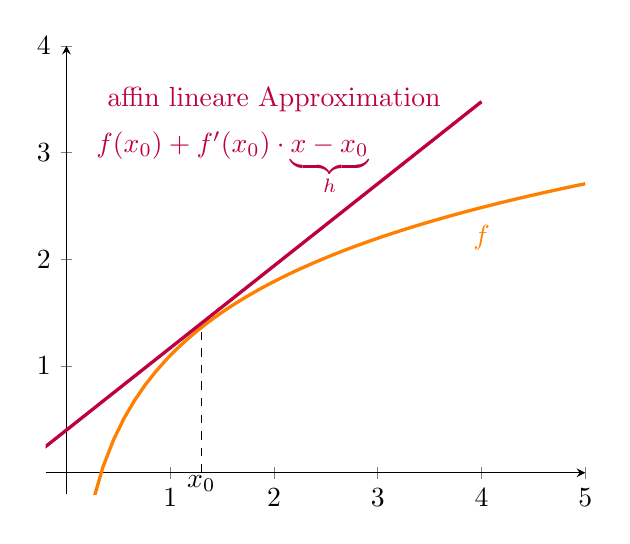
\begin{tikzpicture}
  \begin{axis}[
      axis lines=middle,
      xmax = 5,
      xmin = -0.2,
      ymax = 4,
      ymin = -0.2]
    \addplot [
      domain=-5:5,
      samples=100,
      name path=upper,
      very thick, orange]{ln(3 * x)};
    \node at (1.3,-.1) {$x_0$};
    \node[purple] at (2,3.5) {affin lineare Approximation};
    \node[purple] at (1.6,2.9) {$f(x_0) + f'(x_0) \cdot \underset{h}{\underbrace{x - x_0}}$};
    \node[orange] at (4,2.2) {$f$};
    \addplot [
      domain=-1:4,
      samples=100,
      very thick, purple
    ] {1 / 1.3 * x + 0.4};
    \path[dashed, draw] (1.3,0) -- (1.3, 1.36);
  \end{axis}
\end{tikzpicture}

$X, Y$ normiert, $D \subseteq X$ offen, $f \colon D \to Y$ ist in $x_0 \in D$
Fréchet-differenzierbar $\iff \exists \, T \in \mathcal{L}(X, Y), r \colon X \to Y$
mit
\begin{enumerate}
\item $f(x_0) = f(x_0) + T(h) + r(h)$ \\
  $f(x) = \colorbox{blue!20}{
    $\overset{\text{Affin lineare Approximation}}{\overbrace{f(x_0) + T(x - x_0)}}$
  } + r(x - x_0), x \in D$
\item $\frac{\norm{r(h)}_X}{\norm{h}_X} \overset{h \to 0}\longrightarrow 0$
  bzw. $\frac{\norm{r(x - x_0)}_X}{\norm{x - x_0}_X} \overset{x \to x_0}\longrightarrow 0$
\end{enumerate}
$f'(x_0) \coloneqq T$

\paragraph{Aufgabe 5}
\begin{enumerate}[a)]
\item Für $a, b, c \in \mathbb{R}$ sei $f \colon \mathbb{R} \to \mathbb{R}$
  definiert durch $f(x) \coloneqq ax^2 + bx + c$.
  Geben Sie die Weierstraßsche Zerlegungsformel für ein festes
  $x_0 \in \mathbb{R}$ an.
  Wie lautet $f'(x_0)$?

  \textit{Lsg.}
  Es gilt $f(x_0 + h) - f(x_0) = \qty(a(x_0 + h)^2 + b(x_0 + h) + c)
  - \qty(ax_0^2 + bx_0 + c)$
  $= \underset{h \mapsto (2ax_0 + b)h  \text{ ist linear}}{\underbrace{(2ax_0 + b) \cdot h}} + \underset{r(h)}{\underbrace{h^2}}$

  Es gilt $\abs{\frac{r(h)}{h}} = \frac{h^2}{\abs{h}} = \abs{h} \overset{h \to 0}\longrightarrow 0$

  $\Rightarrow f'(x_0)(h) = \underset{f'(x_0)}{\underbrace{(2ax_0 + b)}} h$

\item Für $A \in \mathbb{R}^{N \times N}, b \in \mathbb{R}^N, c \in \mathbb{R}$ sei
  $f \colon \mathbb{R}^N \to \mathbb{R}$ definiert durch
  \[
    f(x) \coloneqq \left\langle x, Ax \right\rangle + \left\langle b, x \right\rangle + c
  \]
  dabei bezeichne $\left\langle ., . \right\rangle$ das Euklidische Skalarprodukt auf dem $\mathbb{R}^N \colon$
  \[
    \left\langle x, y \right\rangle = \sum_{k = 1}^N x_k y_k \text{ für } x = \qty(x_1, \ldots, x_N), y = \qty(y_1, \ldots, y_N) \in \mathbb{R}^N
  \]
  Wenden Sie die Weierstraßsche Zerlegungsformel an, um $f'(x_0)$ für ein festes
  $x_0 \in \mathbb{R}^N$ zu bestimmen.
  Wie lautet $f'(x_0)$, wenn $A$ eine symmetrische Matrix ist?

  \textit{Lsg.} Es gilt
  $f(x_0 + h) - f(x_0) = \left\langle x_0 + h, A \cdot (x_0 + h) \right\rangle
  + \left\langle b, x_0 + h \right\rangle + c -
  \qty(\left\langle x_0, A \cdot x_0 \right\rangle + \left\langle b, x_0 \right\rangle + c)$

  $= \underset{
    h \mapsto \langle x_0, A \cdot h \rangle + \langle h, A \cdot x_0 \rangle + \langle b, h \rangle \text{ ist linear}
  }{\underbrace{\left\langle x_0, A \cdot h \right\rangle + \left\langle h, A \cdot x_0 \right\rangle
  + \left\langle b, h \right\rangle}} +
  \underset{r(h)}{\underbrace{\left\langle h, A \cdot h \right\rangle}}$

  \fcolorbox{black}{light-gray}{\begin{minipage}{\textwidth}
      \textbf{Cauchy-Schwarzsche Ungleichung}  \\
      Wenn $x, y$ Elemente eines Vektorraumes sind, dann gilt für das
      Skalarprodukt $\langle x, y \rangle$
      \[
        \abs{\langle x, y \rangle} \leq \norm{x} \cdot \norm{y}
      \]
  \end{minipage}}

  Wegen $\frac{\abs{r(h)}}{\norm{h}_2} = \frac{\abs{\left\langle h, A \cdot h \right\rangle}}{\norm{h}_2}
  \leq \frac{\norm{h}_2 \cdot \norm{A \cdot h}_2}{\norm{h}_2} \leq \norm{A} \cdot \norm{h}_2
  \overset{h \to 0}\longrightarrow 0$ ist $f$ in jedem $x_0 \in \mathbb{R}^N$ Fréchet-Differenzierbar
  mit
  \begin{flalign*}
    f'(x_0)(h) &= \langle x_0, A \cdot h \rangle + \langle h, A \cdot x_0 \rangle + \langle b, h \rangle & \\
    &= x_0^T \cdot A \cdot h + h^T \cdot A \cdot x_0 + b^T \cdot h
  \end{flalign*}
\end{enumerate}


\end{document}